\section{Truss Direct Stiffness Method}

% Direct Stiffness Method Resource:
% https://www.colorado.edu/engineering/CAS/Felippa.d/FelippaHome.d/Publications.d/Report.CU-CAS-00-13.pdf

%Assumptions: In a truss external loading is only applied to the joints and there is only axial deformation with no bending.

The \textit{Direct Stiffness Method} is a \textit{Finite Element Method} of analysis that models structural elements as springs. We will begin with deriving the axial stiffness of a structural element. \cite{Felippa2000}

\subsection{Axial Stiffness}
Members in a truss are modelled as springs with only axial deformation. The axial force in the spring is modelled by Hooke's law:

\begin{equation}
	N = k u
\end{equation}

where $N$ is the axial force, $k$ is the axial stiffness, and $u$ is the axial deformation. To define the axial stiffness we will look at a member of constant cross-secitonal area with only elastic deformation. The stress in such a member is defined by the stress-strain relationship:

\begin{equation}
	\sig = E \ep
\end{equation}

where $\sig$ is the stress, $E$ is the modulus of elasticity, and $\ep$ is the strain. Multiplying both sides of the equation by the cross-secional area, $A$, will convert the stress into a force.

\begin{figure}[h]	\centerline{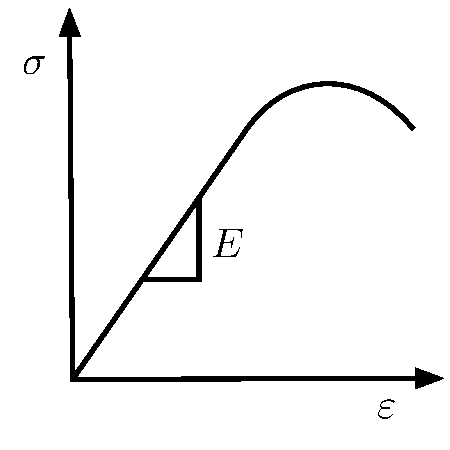
\includegraphics[width=0.5\columnwidth]{Figures/Stress-Strain}}
	\caption{Stress-Strain Relationship}
	\label{fig:Stress-Strain}
\end{figure}

\begin{align}
	\sig A &= E \ep A\\
	N & = E \ep A
\end{align}

The engineering definition of strain will be used here. Strain is defined as:

\begin{equation}
	\ep = \frac{\Delta L}{L_0} = \frac{u}{L}
\end{equation}

where $L$ is the original length of the member and $\Delta L$ is the change in length of the member. Then substituting in the definition of engineering strain into the previous equation:

\begin{align}
	N & = EA \frac{u}{L}
\end{align}

Therefore the axial stiffness from the equation is $\frac{AE}{L}$ for any structural member. The axial force of a structural element can be rewritten as:

\begin{align}
	N & = \frac{AE}{L} u
\end{align}

\subsection{Local Element Stiffness}
Each element in a structural system will have its own local element stiffness equations. The goal of this section will be to develop the local element stiffness equations for a member in matrix form. Taking the nodal equilibrium from figure \ref{fig:LocalMemberStiffness} becomes:

\begin{align*}
	-N &= ku_{1x'}\\
	-N &= ku_{2x'}\\
\end{align*}

Next we will put these equations in matrix form in terms of the local coordinate system. The equation will take the form:

\begin{equation}
	\vec{N} = \vec{k} \vec{u}
\end{equation}

\begin{center}
	\begin{figure}[h]	\centerline{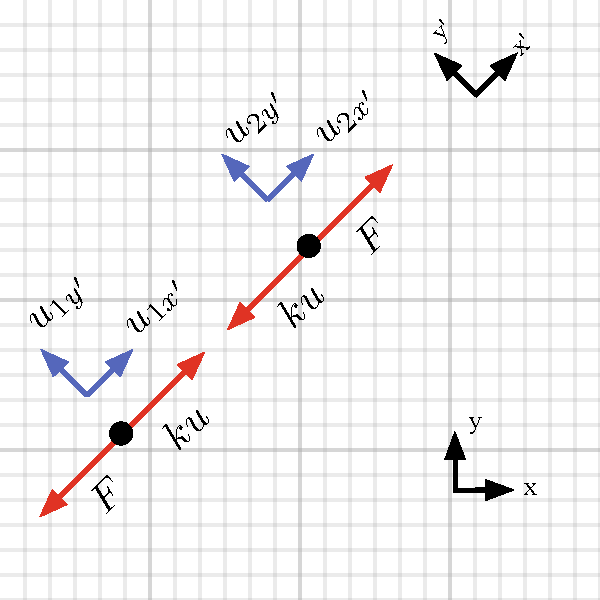
\includegraphics[width=0.7\columnwidth]{Figures/LocalMemberStiffness}}
		\caption{Local Member FBDs}
		\label{fig:LocalMemberStiffness}
	\end{figure}
\end{center}


\begin{equation}
	\underbrace{
		\begin{bmatrix}
			-N\\ 0\\ \hline N\\ 0\\
		\end{bmatrix}
	}_{\vec{N}'}
	=
	\underbrace{
		\frac{AE}{L}
		\begin{bmatrix}
			1 & 0 & -1 & 0\\
			0 & 0 & 0 & 0\\
			-1 & 0 & 1 & 0\\
			0 & 0 & 0 & 0\\
		\end{bmatrix}
	}_{\vec{k}}
	\underbrace{
		\begin{Bmatrix}
			u_{1x'}\\ u_{1y'}\\ \hline u_{2x'}\\ u_{2y'}\\
		\end{Bmatrix}
	}_{\vec{u'}}
	\label{Eq:F=ku}
\end{equation}

Next, we must take the local element stiffness matrix and derive the global element stiffness matrix.

\subsection{Global Element Stiffness}

Transforming local coordinates to global coordinates is described by the following equation:

\begin{equation}
	\begin{Bmatrix}
		u_x\\ u_y
	\end{Bmatrix}
	=
	\underbrace{
		\begin{bmatrix}
			\cos\theta & -\sin\theta\\
			\sin\theta & \cos\theta
	\end{bmatrix}
	}_{\vec{R}}
	\begin{Bmatrix}
		u_x'\\ u_y'
	\end{Bmatrix}
\end{equation}

where $\vec{R}$ is the general rotation matrix. The particular rotation matrix for the two degree of freedom system takes the form:

\begin{equation}
	\vec{T}
	=	
	\begin{bmatrix}
		\vec{R} & \vec{0}\\
		\vec{0} & \vec{R}\\
	\end{bmatrix}
\end{equation}

Note that the values of $\cos\theta$ and $\sin\theta$ can be determined by solving for the $x$ and $y$ component of the element unit vector, respectively. The unit vector can be calculated by:

\begin{align}
	\vec{n} = \frac{\vec{x_2}-\vec{x_1}}{||\vec{x_2}-\vec{x_1}||}
\end{align}

where $\n$ is the unit vector along the element, and $\x_2$ and $\x_1$ are the coordinates of node 1 and node 2, respectively. Now, we take equation \ref{Eq:F=ku}, and multiply both sides of the equation by the local to global transformation matrix, then solve for the axial forces $\vec{N}'$. Note that the global deformation, $\vec{u}$ is equal to $\vec{T}^\intercal \vec{u}$

\begin{align}
	\vec{N}' &= \vec{k} \vec{u}'\\
	\vec{T} \vec{N}' &= \vec{k} \vec{T}^\intercal \vec{u}\\
	\vec{N}' &= \underbrace{\vec{T} \vec{k} \vec{T}^\intercal}_{\vec{k}_{global}} \vec{u}
\end{align}

This gives us the relationship between the global deformation of nodes to the axial force. Enforcing the global nodal boundary conditions will allow solving the system of equations for the member forces. Expanding the equation for $\vec{k}_{global}$ looks like:

\begin{align*}
\vec{k}_{global}
=
\frac{AE}{L}
	\begin{bmatrix}
  		c & -s & 0 & 0\\
  		s & c & 0 & 0\\
  		0 & 0 & c & -s\\
  		0 & 0 & s & c\\
	\end{bmatrix}
	\begin{bmatrix}
  		1 & 0 & -1 & 0\\
  		0 & 0 & 0 & 0\\
  		-1 & 0 & 1 & 0\\
  		0 & 0 & 0 & 0\\
	\end{bmatrix}
	\begin{bmatrix}
  		c & s & 0 & 0\\
  		-s & c & 0 & 0\\
  		0 & 0 & c & s\\
  		0 & 0 & -s & c\\
\end{bmatrix}
\end{align*}

where $c$ and $s$ are $\cos\theta$ and $\sin\theta$, respectively. Therefore the global element stiffness matrix takes the form of:

\begin{equation}
\vec{k}_{global}
=
\frac{AE}{L}
	\begin{bmatrix}
  	c^2 & cs & -c^2 & -cs\\
  	cs & s^2 & -cs & -s^2\\
  	-c^2 & -cs & c^2 & cs\\
  	-cs & -s^2 & cs & s^2\\
	\end{bmatrix}
\end{equation}

Notice that the $\vec{k}_{global}$ matrix is  symetric about the main diagonal. 

\subsection{Global Structural Stiffness}

Deriving the global structural stiffness matrix for a truss is a matter of combining the global element stiffness matricies.

\subsection{Boundary Conditions}

